% !TeX root = ../thuthesis-example.tex

\chapter{引言}

\section{研究问题}
张量可以被用于描述事物之间的线性关系,张量代数则是作用在张量上,对张量所表示关系进行分析的数学工具。
比如在线性系统中,使用二维张量(矩阵)表示系统状态,用矩阵变换表示系统与环境的交互。如果把张量的每个维度看做一种数据,那么张量就可以表示
这些不同种数据之间的关系。比如,在图~\ref{fig:intro}中,利用矩阵乘法即可完成作者引用文章的分析。相似的,社交网络中不同群体的关系,金融计算中不同
交易主体之间的交易信息等,都可以利用张量表示并利用张量代数进行分析。
\begin{figure}
  \centering
  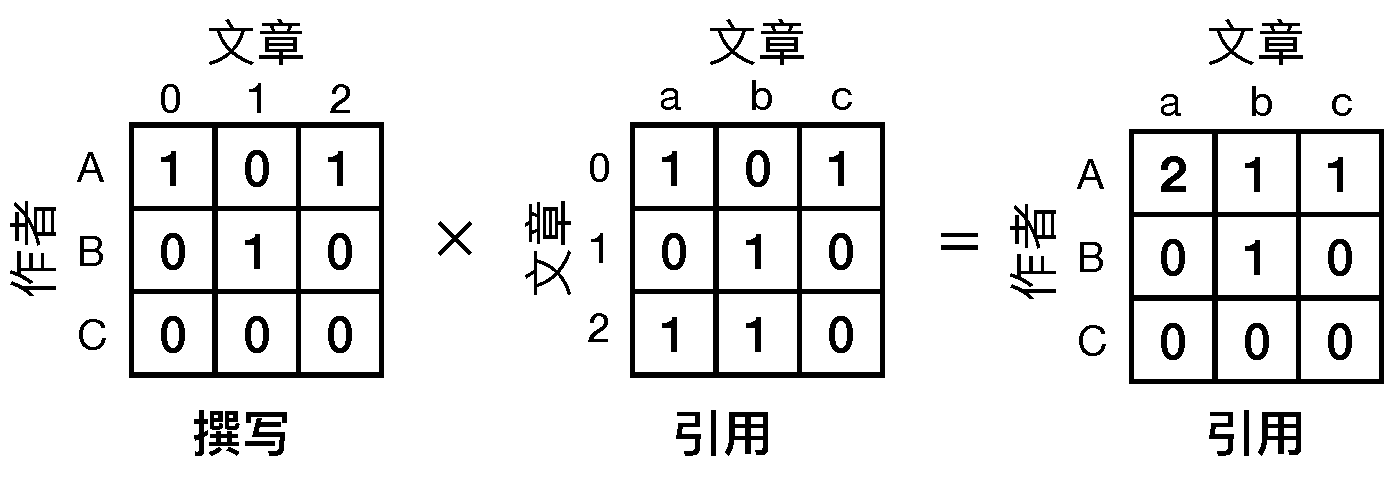
\includegraphics[width=0.9\linewidth]{intro.pdf}
  \caption{稀疏张量代数示例}
  \caption*{第一个矩阵的第一维表示作者,第二维表示文章,矩阵表示的关系是作者写文章。第二个矩阵的第一维表示文章,第二维表示文章,矩阵表示的关系是文章引用文章。
  两个矩阵做矩阵乘法运算后得到的矩阵第一维表示作者,第二维表示文章,关系则变为作者引用文章。}
  \label{fig:intro}
\end{figure}

在现实应用中,因为稀疏关系是普遍存在的\cite{uzzi2007small},所以张量通常是稀疏的。比如在深度神经网络中,不同神经元间连接是稀疏的,体现在权重张量上就是其大部分($50\% \sim 90\%$)可以是零\cite{wang2021dual}。
再比如以及记录亚马逊网站截至2013年3月的横跨18年的用户数据的三维张量中,每一个非零元素对应近80亿个零元\cite{mcauley2013hidden}。
随着稀疏性在神经网络的广泛应用\cite{xiao2022smoothquant},以及现实生活中关系数据的日益增长,需要研究更高效的稀疏张量运算。

稀疏计算在系统中处于算子层面。如图~\ref{fig:kernel-def}所示,算子的功能是连接算法和硬件,是高效计算系统的核心。因此,稀疏计算的优化核心是稀疏算子。
\begin{figure}
  \centering
  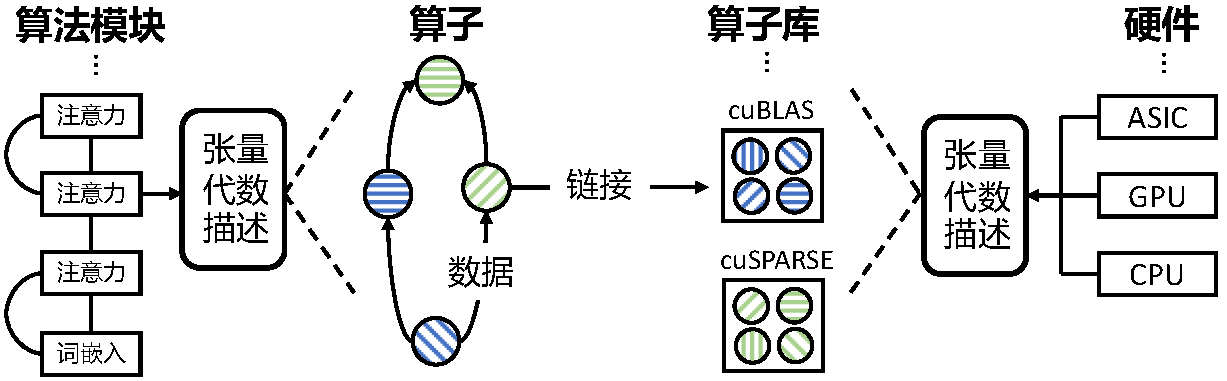
\includegraphics[width=0.9\linewidth]{kernel-def.pdf}
  \caption{算子在计算系统的位置}
  \caption*{以Transformer算法\cite{vaswani2017transformer}为例介绍算子在计算系统中的位置。词嵌入和注意力是Transformer算法的基础模块。Tranformer算法主体是重复的注意力模块。注意力模块通过张量代数描述可以转化为多个算子的运算组合。这种组合可以用有向无环图表示,其中边代表数据,点代表算子。
  图中点的不同花纹代表不同算子,不同颜色代表属于不同算子库。硬件厂商会提供以张量代数描述定义的算子库。每个算子库包含一类算子,完成提前定义的张量代数运算。比如图中cuBLAS\cite{cuBLAS}是英伟达GPU的线性代数算子库,cuSPARSE\cite{naumov2010cusparse}是英伟达GPU的稀疏线性代数算子库。系统在实际运行时,会根据算法模块需求通过链接技术调用算子库中的对应算子。}
  \label{fig:kernel-def}
\end{figure}
然而,稀疏算子在优化技术和开发成本上仍面临挑战。一方面,由于稀疏计算的不规则性,在当前主流并行计算平台上的高效算法的研究仍不充分。另一方面,由于稀疏计算在代数表达和优化技巧方面的多样性,当前稀疏算子库模式开发成本过高。

虽然GPU提供了10TFLOP/s量级的并行计算能力,但是由于稀疏张量计算的不规则性,充分利用GPU的并行计算能力仍具有挑战性。表\ref{tab:motivation-1}展示了SDDMM\cite{yu2021exploiting},SpMM\cite{huang2020ge},MTTKRP\cite{nisa2019mttkrp},其中每种算子均采用当前性能最高的开源库。
\begin{table}
  \centering
  \caption{稀疏张量算子库性能和GPU峰值算力对比}
  \begin{tabular}{llll}
    \toprule
    算子名  & 算子性能(TFLOP/s) & 平台峰值算力(TFLOP/s) & 与峰值算力差距倍数   \\
    \midrule
    SDDMM  & 0.42 & 15.7 & 37.4x \\
    SpMM   & 0.28 & 10.6 & 37.9x \\
    MTTKRP & 0.20 & 15.7 & 78.5x \\
    \bottomrule
  \end{tabular}
  \label{tab:motivation-1}
\end{table}
从表\ref{tab:motivation-1}中可以看出,最佳的开源稀疏张量算子库算子性能和平台峰值算力还有几十倍的差距,这说明计算平台的算力还没有被充分利用。因此主要挑战是如何进一步扩展优化空间,即写出更高效的稀疏张量算子。

除了算子性能较低,现在编写高性能稀疏算子库也较为困难。这里用代码行数来衡量编写算子库的难易程度。表\ref{tab:motivation-2}展示了SDDMM,SpMM,MTTKRP最佳算子库和稀疏张量编译器TACO的对比。其中算子库代码行数指编写GPU上执行的CUDA算子需要的代码行数(不包括CPU和GPU间数据搬移和算子调用的代码),算子编译器代码行数指运用TACO提供的调度变换指令编写算子所需要的代码行数。
\begin{table}
  \centering
  \begin{threeparttable}[c]
  \caption{稀疏张量算子库和算子编译器的性能和代码行数对比}
  \label{tab:motivation-2}
  \begin{tabular}{lllll}
    \toprule
    算子名  & 算子库 & 算子编译器 & 算子库与编译器 & 算子库与编译器   \\
           & 代码行数 & 代码行数 & 代码行数比    & 算子性能比       \\
    \midrule
    SDDMM\tnote{a}  & 53 & 12 & 4.4x & 2.1x \\
    SpMM\tnote{b}   & 132 & 13 & 10.2x & 2.6x \\
    MTTKRP\tnote{c} & 40 & 12 & 3.3x & 1.2x \\
    \bottomrule
  \end{tabular}
  \begin{tablenotes}
    \item [a] 选取SOTA的GPU开源SDDMM算子库 PRedS \cite{yu2021exploiting}中的sddmm\_csr\_ebalance\_vec4函数和TACO中的scheduleSDDMMGPU函数做对比。
    \item [b] 选取SOTA的GPU开源SpMM算子库 DASpMM \cite{dai2022heuristic}中的采用的四种算子:csrspmm\_rowcaching\_rowbalance\_kernel,
      csrspmm\_rowcaching\_nnzbalance\_kernel,csrspmm\_parreduce\_rowbalance\_kernel和csrspmm\_parreduce\_nnzbalance\_kernel函数的平均行数和TACO中的scheduleSpMMGPU函数对比。
    \item [c] 选取SOTA的GPU开源MTTKRP算子库MM-CSF\cite{nisa2019mttkrp}中采用HyB格式的3维MTTKRP函数的平均行数和TACO中的scheduleMTTKRPGPU函数对比。
  \end{tablenotes}
  \end{threeparttable}
\end{table}
从表\ref{tab:motivation-2}中可以看出,利用编译器提供的领域专用语言可以减小3到10倍的代码量,但是会牺牲16\%到60\%的性能。性能下降说明编译器表达的优化空间没有包含已有算子库的优化技巧。
因此,需要设计更好的编译算法,在进一步降低用户代码量的同时,扩展优化空间,从而使得用户可以用更低的开发难度得到更高性能的稀疏张量算子。

\section{本文贡献}
本文针对算子性能低的问题提出新的算子优化技术,并针对优化技巧在不同稀疏张量运算的迁移问题提出更高效的稀疏编译算法,在提升算子性能同时降低部署复杂度。贡献总结如图~\ref{fig:contrib}。

本文提出了灵活规约优化技术,这是一种新的针对SIMT架构上稀疏稠密混合张量代数算子优化技术。该技术扩展了优化空间,进一步提升了算子库性能。实验表明,采用灵活规约同步后可以将SpMM算子库性能提升平均1.6至2.3倍(针对不同代GPU架构加速比有所不同)。

基于灵活规约优化技术,本文提出了灵活规约语义提升技术,这是一种新的针对SIMT架构上稀疏稠密混合张量代数的编译算法。该技术扩展了稀疏算子编译器表达的优化空间,同时在用户端只需要增加一行代码即可获得灵活规约带来的算子加速。
实验表明,采用该技术后,编译器生成SpMM算子性能提升了平均1.2倍,最多提升3.8倍;编译器生成MTTKRP算子性能最多提升2.7倍。

\begin{figure}
  \centering
  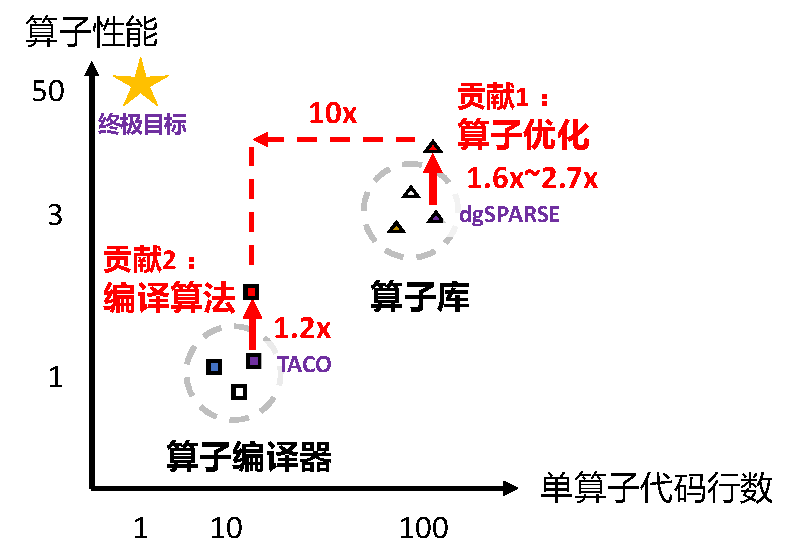
\includegraphics[width=0.7\linewidth]{contrib.pdf}
  \caption{本文贡献总结}
  \label{fig:contrib}
\end{figure}

\section{本文框架}
本文第2章介绍了稀疏稠密混合代数,针对GPU上稀疏稠密混合代数的优化技术,以及稀疏算子编译器的背景知识和相关工作。第3章阐释了灵活规约的内涵,构建了基于灵活规约的
扩展优化空间,并通过实验验证了灵活规约的有效性,探讨了优化空间的结构。第4章阐述了灵活规约语义提升技术的定义,介绍了算法流程和系统部署,并通过实验验证了编译算法针对稀疏稠密混合代数优化的有效性。第5章总结了本文的工作,
并为未来算子编译器研究提出可能的研究问题。
